% vim: set spelllang=fr:
\chapter{Annotation en rôles sémantiques fondée sur la connaissance}
\label{ch:srl}


%\citep{simmons1973semantic} is the earliest work on Semantic Role Labeling.
%Already based on \citep{fillmore1968case}, it parsed a sentence into what we
% know call semantic roles. (check)

%Contrairement aux autres ressources pour l'annotation en rôles sémantiques,
%VerbNet couvre l'ensemble des verbes fréquents du vocabulaire tout en étant
%conçu sur des préceptes robustes le rendant utile pour les tâches de Traitement
%Automatique des Langues (Section~\ref{ch:verbnet:sec:verbnet}).

La tâche d'annotation en rôles sémantiques a reçu beaucoup d'attention ces
dernières années, à la fois pour les approches supervisées et semi-supervisées.
Les approches fondées sur la connaissance, elles, ne se basent pas sur des
corpus annotés mais sur des ressources lexicale existantes. Ce type d'approche
a été négligé malgré leur complémentarité par rapport aux autres approches.

En nous inspirant de \citep{swier2004unsupervised,swier2005exploiting}, nous
montrons dans ce chapitre un système d'annotation en rôles sémantiques fondé
sur la connaissance qui se veut simple à mettre en place et facile à
reproduire. Dans ce système, la prise en compte de la voix passive réduit le
taux d'erreur de 15,7~\%, ce qui montre la marge de progrès existante. Malgré
des performances moindres quand des données d'entraînement existent, l'approche
facilite l'analyse des erreurs, n'a pas besoin d'un corpus annoté manuellement
et est a priori indépendante du domaine considéré, ce qui sera étudié plus en
détail dans le Chapitre~\ref{ch:domainsrl} où les domaines du football, du
réchauffement climatique et de l'informatique seront considérés.

Ce chapitre se concentre sur notre système d'annotation en rôles sémantiques
dans un cadre général en l'utilisant sur le corpus FrameNet anglais (qui a été
présenté à la section~\ref{presentation_framenet}). Les chapitres suivants
montreront la versatilité de ce système dans des contextes différents : en
domaine spécifique (Chapitre~\ref{ch:domainsrl}) et pour le français
(Chapitre~\ref{ch:frenchsrl}).

\section{Tâche}

L'objectif de ce chapitre est de présenter notre système en l'évaluant sur le
corpus annoté en rôles sémantiques fourni par FrameNet, ce qui permet une
comparaison avec les approches existantes. La figure~\ref{fig:srlrussia} est un
exemple d'annotation en rôles sémantiques avec des frames et des rôles
FrameNet. Nous utiliserons principalement cette phrase d'exemple par la suite
pour illustrer notre propos. Pour une phrase donnée, les prédicats verbaux et
la frame qu'ils évoquent sont identifiés. Dans chaque phrase, des syntagmes
vont remplir un des rôles prévus par la frame dans FrameNet. Ces syntagmes sont
nommés «~remplisseurs de rôle~» (\emph{role filler} en anglais).

\begin{figure}[ht]
    \begin{quote}
    However, in 2002 Russia declared it will eliminate its tactical nuclear weapons by the end of 2004.
    \end{quote}

    L'objectif est d'aboutir à la représentation suivante :

    \begin{itemize}
        \item \emph{declare} déclenche la frame Statement dont les rôles sont remplis ainsi :
        \begin{itemize}
            \item Speaker : Russia
            \item Message : it will eliminate its tactical nuclear weapons by the end of 2004
            \item Time : in 2002
        \end{itemize}
        \item \emph{eliminate} déclenche la frame Removing dont les rôles sont remplis ainsi :
        \begin{itemize}
            \item Agent: it
            \item Theme: its tactical nuclear weapons
            \item Source: \emph{non instancié}
        \end{itemize}
    \end{itemize}
    \caption{\label{fig:srlrussia}Exemple d'annotation en rôles sémantiques}
\end{figure}

Toute interprétation supplémentaire non présente dans la
figure~\ref{fig:srlrussia} est en dehors du cadre de l'annotation en rôles
sémantiques, ce qui est la raison pour laquelle la tâche est aussi connue sous
le nom d'analyse sémantique de surface (\emph{shallow semantic parsing}).  Il
est néanmoins intéressant de garder à l'esprit les applications possibles de
tels travaux. Par exemple, un système de question-réponse pourrait utiliser la
représentation de ces deux \emph{frames} pour répondre à la question \emph{Does
Russia possess tactical nuclear weapons?} L'annotation de la
figure~\ref{fig:srlrussia} est une information utile, mais elle ne serait pas
suffisante pour répondre à la question : il faut aussi comprendre la question,
annoter les coréférences (\emph{it} fait référence à \emph{Russia}), établir la
crédibilité du \emph{Speaker}, s'intéresser à d'autres phrases potentiellement
contradictoires, etc.

\section{Système}

Le système présenté est similaire à celui de
\cite{swier2004unsupervised,swier2005exploiting}. Cependant, dix ans après, il
est important d'évaluer à nouveau cette approche pour savoir où elle se situe
par rapport à l'état de l'art et pour proposer certaines améliorations.

Pour commencer, chaque phrase à annoter doit d'abord être étiquetée en
morphosyntaxe et analysée syntaxiquement. Nous laissons ici ces analyses à des
systèmes externes présentés à la section~\ref{subsec:details_exp}. C'est
l'entrée de notre système, la sortie étant l'annotation en rôles sémantiques
montrée dans la figure~\ref{fig:srlrussia}.

Ensuite, nous utilisons les informations de VerbNet (présenté à la
section~\ref{presentation_verbnet}) sur l'interface entre la syntaxe et la
sémantique. Dans VerbNet, chaque classe regroupe un certain nombre de verbes
acceptant certaines constructions syntaxiques. Les syntagmes participant à ces
constructions sont associés à des rôles sémantiques à interpréter dans le
contexte de la classe.  Nous notons ces constructions NP.Agent V NP.Theme, ce
qui indique que dans cette constructions transitive (NP V NP, e.g. \emph{Sally
pushed the chair}), le premier syntagme nominal (\emph{Sally}) est Agent alors
que le second (\emph{the chair}) est Theme. L'interprétation des rôles, ici
Theme et Agent, dépend de la classe VerbNet considérée. Par exemple, dans la
classe \texttt{resign-10.11}, l'Agent est la personne qui démissionne et la
Source est le poste qui a été quitté.

Pour une phrase donnée, le système commence par identifier les verbes de
cette phrase. Pour chacun de ces verbes, un ensemble de classes VerbNet est
identifié. Ainsi, pour notre phrase d'exemple ci-dessus, les classes possibles
pour le verbe \emph{declare} sont \texttt{declare-29-4-1-1-1},
\texttt{say-37.3-1} et \texttt{reflexive\_appearance-48.1.2}. Le choix correct
est \texttt{say-37.3-1}, mais il n'est pas possible de le déterminer avant de
considérer les frames listées par VerbNet dans ces différentes classes.

Par exemple, \texttt{reflexive\_appearance-48.1.2} contient la frame NP.Agent V
NP.Theme. Ainsi, si un des verbes de cette classe, tel que \emph{present} :
\begin{itemize}
    \item est utilisé dans un sens compatible avec la classe
        \texttt{reflexive\_appearance-48.1.2},
    \item et est utilisé avec un sujet syntagme nominal et un objet syntagme
        nominal,
\end{itemize}
alors le sujet du verbe est l'Agent et l'objet est le Theme.

La phrase d'exemple de la figure~\ref{fig:srlrussia} ne correspond pas à NP V
NP mais à NP V that S (\emph{that S} étant la notation VerbNet pour les
complétives introduites par \emph{that}). La seule occurrence de cette frame
VerbNet est dans \texttt{say-37.7-1} : NP.Agent V that S.Topic (\emph{He
ordered that he go}). Les classes \texttt{declare-29-4-1-1-1} et
\texttt{reflexive\_appearance-48.1.2} ne listant pas cette frame, il est
possible d'établir que :

\begin{itemize}
    \item la classe VerbNet qui convient est \texttt{say-37.7-1},
    \item \emph{Russia} est Agent,
    \item \emph{it will eliminate its tactical nuclear weapons by the end of 2004} est Topic.
\end{itemize}

Enfin, le mapping entre VerbNet et FrameNet (section~\ref{sec:mapping}) nous
informe que :

\begin{itemize}
    \item la classe VerbNet \texttt{say-37.7} correspond à la frame Statement,
    \item dans cette classe, le rôle VerbNet Agent correspond au rôle FrameNet Speaker,
    \item dans cette classe, le rôle VerbNet Topic correspond au rôle FrameNet Topic.
\end{itemize}

Nous aboutissons ainsi pour le verbe \emph{eliminate} à la représentation
voulue pour notre phrase d'exemple.

On ne peut pas toujours identifier la classe VerbNet correcte. C'est le cas par
exemple de \texttt{reflexive\_appearance-48.1.2} et \texttt{say-37.3-1} qui
contiennent toutes les deux le cadre NP V NP. Sans corpus annoté, ces
ambiguïtés ne peuvent pas être résolues.  Cependant, une fois qu'une première
série de correspondances a été effectuée, il est possible d'utiliser les
connaissances du domaine étudié pour annoter de nouveaux syntagmes nominaux
(section~\ref{subsec:probability}).

Les sections suivantes décrivent le déroulement précis de l'algorithme en le
découpant en quatre étapes.

\subsection{Identification du prédicat}

Chaque phrase peut contenir un ou plusieurs prédicats : nous nous contentons
ici de retenir tous les verbes ayant été annotés avec les parties du discours
acceptées et présents dans VerbNet. Les autres prédicats potentiels,
c'est-à-dire ceux qui ne sont pas dans VerbNet et ne sont pas des verbes, sont
ignorés. Les parties du discours acceptées sont md, MD, VB, VBD, VBG, VBN, VBP,
VBZ, VV, VVD, VVG, VVN, VVP, VVZ, VH, VHD, VHG, VHN, VHP et VHZ.
% TODO la liste est différente dans argguesser.py/argheuristic.py

\subsection{Identification des arguments}

% TODO tagset syntaxique WSJ
Cette étape identifie les syntagmes amenés à jouer un rôle sémantique lors de
l'annotation. Nous suivons ici \cite{lang2011unsupervised} qui propose huit
règles\footnote{La septième règle n'est pas utilisée.} basées sur l'analyse
syntaxique de la phrase. Initialement, tous les mots sont candidats. Puis
chacune de ces règles sélectionne ou écarte des mots candidats. Dans la
représentation en dépendances, si le mot sélectionné est la tête d'un syntagme,
c'est le syntagme entier qui devient candidat. Sinon, c'est uniquement le mot.
Les règles appliquées dans l'ordre sont :

\begin{enumerate}
    \item Éliminer les déterminants, les marqueurs d'infinitifs, les conjonctions de coordinations et la ponctuation.
    \item Éliminer les candidats dont le chemin du prédicat au candidat finit par une coordination, une subordination, etc.
    \item Conserver les candidats qui sont les sujets les plus proches à gauche du prédicat et dont les relations du prédicat p à la tête t du candidat sont toutes montantes (g -> p)
    \item Éliminer les candidats  dont le chemin entre le prédicat et le candidat, sauf la dernière relation, contient une relation de sujet, une relation de modifieur adjectival, etc.
    \item Éliminer les verbes auxiliaires
    \item Conserver les candidats directement sous le prédicat
    \item \sout{Conserver les candidats si le chemin du prédicat au candidat traverse plusieurs noeuds verbaux}
    \item Éliminer tous les candidats restants.
\end{enumerate}

% TODO exemple
Pour les règles 3 et 4, la liste complète des relations acceptées est listé en
annexe à la section~\ref{argument_identification}. En pratique sur le corpus
FrameNet, ces règles génèrent des candidats qui ne jouent pas de rôle : notre
système devra par la suite pouvoir écarter ces candidats tout en assignant les
rôles corrects aux candidats qui jouent bien un rôle.

Cette étape d'identification des arguments est facultative : afin de mieux
comprendre les performances des étapes suivantes, ce seront parfois les
arguments parfaits de la vérité-terrain qui seront utilisés lors de
l'évaluation. En effet, l'objectif est d'évaluer l'apport de VerbNet à la tâche
de l'annotation en rôles sémantiques, et l'identification des arguments, bien
qu'une partie intégrante de tout système complet d'annotation en rôles
sémantiques \citep{das2010probabilistic}, ne fait pas partie de nos
contributions.

\subsection{Correspondance exacte des frames}

Cette étape associe zéro, un ou plusieurs rôles sémantiques à chaque syntagme
candidat identifié lors de l'étape précédente.

Nous incluons ici deux étapes traditionnellement utilisées dans les systèmes
d'annotation en rôles sémantiques \citep{gildea2002automatic,das2014frame} :
l'identification des frames FrameNet puis l'assignation de rôles aux arguments
identifiés. Ici, au contraire, ce sont les contraintes syntaxiques définies
dans les frames VerbNet qui permettent de restreindre les classes VerbNet
possibles. Une fois la frame identifiée syntaxiquement, les rôles peuvent être
attribués aux syntagmes.

Premièrement, les syntagmes candidats sont représentés au format VerbNet. Par
exemple, si trois syntagmes nominaux ont été identifiés comme arguments, dont
un avant le verbe, la représentation VerbNet de la phrase devient NP V NP NP.
Pour comparer la représentation VerbNet de la phrase aux frames VerbNet, nous
identifions toutes les classes VerbNet incluant le prédicat.

Par exemple, le prédicat \emph{classify} est présent dans deux classes
VerbNet~: \texttt{characterize-29.2} et \texttt{classify-29.10}. Les frames
possibles sont~:

% TODO séparer par classe, on doit pouvoir suivre la suite sans regarder
% VerbNet
\begin{itemize}
    \item NP.Agent V NP.Theme (as) S\_ING.Attribute
    \item NP.Agent V NP.Theme to be ADJ.Attribute
    \item NP.Agent V NP.Theme as PP.Attribute
    \item NP.Agent V NP.Theme
    \item NP.Agent V NP.Theme as PP.Goal
    \item NP.Agent V NP.Theme in PP.Location
\end{itemize}
% TODO documenter la gestion des PP - demande de savoir comment on unifie avec
% domainsrl

% TODO trouver une telle phrase dans FrameNet ?
Considérons la phrase \emph{The curator classified the artifacts}. La
représentation VerbNet de cette phrase est NP V NP, ce qui correspond au
NP.Agent V NP.Theme de la classe \texttt{classify-29.10}. On en déduit que
\emph{The curator} est Agent, et que \emph{the artifacts} est Theme. Cette
phrase est donc correctement annotée en rôles sémantiques VerbNet.

Prenons un autre example, cette fois tiré de FrameNet. La phrase \emph{The
company also classifies short and wide radius ruts according to their severity}
est transformée en NP V NP according PP. Dans ce cas, seuls les deux premiers
syntagmes peuvent être mis en correspondance avec les frames VerbNet listées
ci-dessus. Il n'y a pas de correspondance possible pour le troisième syntagme:
VerbNet n'encode pas \emph{according} comme une préposition possible alors que
\emph{in} et \emph{as} sont acceptées. De tels arguments non prévus pas VerbNet
ne sont pas annotés lors de cette étape. C'est ici un problème de couverture.
Les auteurs de VerbNet travaillent actuellement sur la couverture de la
ressource en ajoutant des informations syntaxiques et lexicales issues de très
larges corpus \citep{bonial2013expanding}. Le résultat de ces travaux n'est
cependant pas disponible dans la version 3.2 de VerbNet que nous utilisons. Ce
problème de couverture empêche d'assigner la classe VerbNet qui convient. Par
conséquent, même si on sait que quelle que soit la classe, le sujet serait
Agent et le premier objet Theme, cette information n'est pas utile parce qu'on
ne sait pas comment l'interpréter.

\subsection{Correspondances probabiliste des frames}
\label{subsec:probability}

Maintenant que les correspondances exactes ont étés effectuées, il reste les
correspondances ambigües pour lesquelles plusieurs frames sont possibles.  Nous
pouvons utiliser les frames déjà mises en correspondance pour annoter ces
frames ambigües. La méthode reste non supervisée : bien que nous entraînions
une forme simple d'algorithme supervisé, nous le faisons sur des données non
annotées simplement obtenues de manière automatique sur le corpus existant.
Nous faisons ici l'hypothèse qu'un corpus entier est à annoter, mais dans le
cas où l'annotation se ferait phrase par phrase, il serait possible
d'abandonner cette étape ou d'alimenter les classifieurs que nous utilisons au
fur et à mesure des annotations.

L'apprentissage se fait sous la forme d'un simple classifieur statistique. Deux
classifieurs sont utilisés : le premier détermine la classe VerbNet quand
celle-ci est ambigüe, et le second détermine le rôle d'un syntagme quand
plusieurs choix sont possibles.

% TODO on peut avoir un modèle pour identifier la classe VerbNet
Le premier classifieur est à implémenter absolument...

Le second classifieur (issu de \cite{swier2004unsupervised}) assigne une
probabilité aux différents rôles possibles en s'aidant des rôles déjà
identifiés.

% TODO belles formules comme dans gildea2002automatic
$$ \text{rôle} = \arg\max_{\text{rôle}} p(\text{rôle} \vert \text{prédicat}, \text{fonction})$$

La fonction est la fonction grammaticale identifiée d'après l'analyse
syntaxique : si un syntagme apparaît avant le verbe, il est sujet, si il est
après le verbe, et il est objet, et ainsi de suite. Les syntagmes
prépositionnels sont traités à part : la préposition qui introduit le syntagme
est considérée à part.

Ce classifieur utilise l'information du prédicat et la fonction grammaticale
détectée. Par exemple, dans notre corpus (section~\ref{subsec:details_exp}),
l'objet direct du verbe 'négliger' est le plus souvent 'Theme'.

La précision pour ce modèle est forte, mais il n'assigne des rôles que pour
40~\% des arguments : dans les autres cas, nous ne disposons pas d'informations
pour cette paire (prédicat, fonction grammaticale).

\section{Mapping VerbNet - FrameNet}
\label{sec:mapping}

% TODO principe
% TODO difficultés à réaliser un tel mapping
% TODO impliquant des limites
% TODO parfait ?

\section{Gestion de la voix passive}
\label{sec:passif}

Une analyse d'erreur a révélé que la voix passive était une source d'erreur
importante dans l'analyse de notre corpus FrameNet. En effet, VerbNet n'encode
pas la voix passive qui est un phénomène syntaxique : c'est au moment de
l'analyse syntaxique que les sujets et objets syntaxiques, profonds ou non,
doivent être identifiés correctement. Pour annoter la phrase \emph{The
artifacts were classified by the curator} en rôles sémantiques, il est donc
important de d'abord transformer la phrase en \emph{the curator classified The
artifacts} avant la comparaison les frames VerbNet.

Les sujets et objets profonds ne sont pas encodés dans les corpus annotés en
syntaxe que nous utilisons (le Wall Street Journal pour l'anglais, cf.
section~\ref{subsec:details_exp}). Une étape intermédiaire est donc nécessaire
entre l'analyse syntaxique et l'annotation en rôles sémantiques
\citep{bonfante2011modular, ribeyre2013systeme}. Cette étape intermédiaire
pourra identifier les sujets et objets profonds de tous les verbes considérés,
évitant ainsi des erreurs lors de l'annotation en rôles sémantiques. 

Afin de valider cette hypothèse, nous nous sommes concentrés sur la voix
passive qui était le phénomène de syntaxe profonde le plus présent dans notre
corpus.  Pour annoter les verbes utilisés avec la voix passive, nous avons
transformé les frames VerbNet vers la voix passive. Les verbes utilisés au
passif en anglais sont au participe passé et gouvernés par une forme du verbe
\emph{to be}. Étant donné une frame VerbNet telle que \emph{NP.Agent V
NP.Recipient NP.Theme}, nous la remplaçons par deux nouvelles frames :

\begin{itemize}
    \item NP.Recipient V NP.Theme
    \item NP.Recipient V NP.Theme by NP.Agent
\end{itemize}

Ce sont ces frames VerbNet transformées qui sont utilisées lorsque qu'une voix
passive est detectée, ce qui améliore les résultats
(Table~\ref{table:results}). Cette expérience valide la gestion de tels
phénomènes syntaxiques. Pour aller plus loin, il faudra non pas modifier
VerbNet mais bien annoter la phrase en syntaxe profonde avant de réaliser les
correspondances exactes puis probabilistes.

\section{Evaluation}
\label{srl:evaluation}

L'intérêt du système ne réside pas dans l'annotation d'un large corpus annoté
tel que FrameNet pour lequel les méthodes d'apprentissage supervisées sont les
plus efficaces \citep{das2014frame}. En effet, notre méthode est destinée à
annoter de nouveaux domaines ne disposant pas de corpus annoté
(Chapitre~\ref{ch:domainsrl}). Néanmoins, FrameNet est un point de comparaison
utilisé par de nombreux systèmes d'annotation en rôles sémantiques auxquels il
est intéressant de se comparer.

% TODO mettre avant mention dans 6.2
FrameNet et VerbNet n'utilisant ni la même séparation en rôles ni la même
séparation en classes, nous utilisons le mapping VerbNet-FrameNet maintenu par
le projet SemLink.

Le corpus FrameNet est équilibré et inclut des textes de diverses sources : le
Wall Street Journal, les corpus AQUAINT et MASC, ainsi que d'autres textes
divers.

\subsection{Détails expérimentaux}
\label{subsec:details_exp}

FrameNet dispose de deux corpus. Le premier corpus est le corpus d'exemples :
des phrases tirées du British National Corpus illustraient la diversité de
réalisation des frames annotés. Plus tard, les versions 1.3, 1.4 et 1.5 de
FrameNet ont apporté un corpus dit full-text, plus adapté à la tâche
d'annotation en rôles sémantiques : au lieu d'identifier des exemples pour
toutes les frames, tous les prédicats présents dans un texte donné sont annotés
en rôles sémantiques. Ici, nous utilisons le corpus full-text de FrameNet 1.5
et pas le corpus d'exemples.

Nous utilisons VerbNet 3.2 et le mapping VerbNet-FrameNet 1.2.2c
\footnote{\url{http://verbs.colorado.edu/semlink/1.2.2c/vn-fn/}}. Notre système
n'annote que les arguments Core étant donné que ce sont généralement les
arguments étudiés par VerbNet.

% TODO de toute façon il faut utiliser ce qui est fourni par SEMAFOR
Pour la tâche complète qui inclut l'identification des arguments, nous
utilisons le parser MST dans sa version 0.5.0 \citep{mcdonald2006multilingual}
entraîné sur une version modifiée du Wall Street Journal de la manière
suivante. Nous avons d'abord transformé l'encodage des syntagmes nominaux
\footnote{\url{http://sydney.edu.au/engineering/it/~dvadas1/}}
\citep{vadas2007adding} puis appliqué l'outil de conversion
constituants-dépendances du LTH pour une conversion au format CoNLL
\footnote{\url{http://nlp.cs.lth.se/software/treebank_converter/}}
\citep{johansson2007extended}. De plus, FrameNet incluant des parties du corpus
du Wall Street Journal, nous avons supprimé les fichiers 0558, 0089, 0456,
1778, 1286 et 1695 du corpus d'entraînement de l'analyseur syntaxique. Ceci
évite que l'analyseur traite des phrases déjà observées dans le corpus
d'entraînement, ce qui aurait pu améliorer les résultats artificiellement.

Enfin, les étiquettes morphosyntaxiques de FrameNet, utilisées lors de
l'analyse syntaxique, ont été converties de la convention BNC à la convention
WSJ en utilisant des règles manuelles (Table~\ref{table:tagset_rules}). Sur les
six fichiers du Wall Street Journal pour lesquels on connaît l'annotation
correcte au format WSJ, ceci réduit les erreurs de 23\% à 3\%.

\begin{table}[ht]
    \centering
    \begin{tabular}{ccc|ccc}
        \toprule
        JJ   &$\to$& ADJ    & JJR  &$\to$& NP     \\
        JJS  &$\to$& NP     & MD   &$\to$& S      \\
        NN   &$\to$& NP     & NNP  &$\to$& NP     \\
        NNPS &$\to$& NP     & NNS  &$\to$& NP     \\
        NP   &$\to$& NP     & NPS  &$\to$& NP     \\
        PP   &$\to$& PP     & PRP  &$\to$& NP     \\  
        RB   &$\to$& ADV    & TO   &$\to$& to S   \\
        VB   &$\to$& S      & VBD  &$\to$& S      \\
        VBG  &$\to$& S\_ING & VBN  &$\to$& ADJ    \\
        VBP  &$\to$& S      & VBZ  &$\to$& S      \\
        WDT  &$\to$& NP     & \$   &$\to$& NP     \\  
        CD   &$\to$& NP     & DT   &$\to$& NP     \\
        \bottomrule
    \end{tabular}
    \caption{\protect\centering\label{table:tagset_rules}Règles de conversion entre les parties du discours BNC et WSJ}
\end{table}

% FUTURE SEMAFOR MXPOST/MST

\subsection{Procédure d'évaluation}

\begin{table*}[ht]
    \centering
    \begin{tabular}{lcccc}
        \toprule
        Task                                           & F1        & Accuracy \\
        \midrule
        FM                                             & 70.48\%   & 53.09\%  \\
        FM + prédicat-fonction (gold args)                & 72.02\%   & 58.28\%  \\
        FM + passif + prédicat-fonction (gold args)      & 76.40\%   & 62.72\%  \\
        \midrule
        Identification + FM                            & 46.75\%   & 29.12\%  \\
        Identification + FM + prédicat-fonction           & 46.78\%   & 33.49\%  \\
        \bottomrule
    \end{tabular}
    \caption{\protect\centering\label{table:results}Résultats pour différentes tâches. FM est le frame matching. \emph{passif} indique la détection de la voix passive. \emph{Identification} est l'identification des arguments.}
\end{table*}

Les rôles annotés de chaque phrase FrameNet sont d'abord transformés en rôles
VerbNet. Pour chaque classe FrameNet, un rôle FrameNet peut correspondre à 0, 1
ou plusieurs rôles VerbNet :

\begin{itemize}

    \item zéro : n'y pas de correspondance pour les frames FrameNet trop éloignées
    des classes VerbNet. C'est un problème répandu :  seulement 4605 rôles sur les
    10052 rôles présents dans FrameNet ont au moins une association VerbNet.
    % TODO Cependant, en pratique, dans le corpus FrameNet, XX~\% des occurrences
    % de rôles sont associées à plus d'un rôle VerbNet

    \item plusieurs : il y a plusieurs correspondances quand un rôle FrameNet
    est ambigu par rapport à un rôle VerbNet. Les rôles FrameNet étant définis plus
    précisément, c'est un problème rare. % TODO dans quelle mesure ?

\end{itemize}

Dans tous les autres cas, un rôle FrameNet correspond à un rôle VerbNet unique,
et c'est ce rôle VerbNet que notre système doit déterminer. Nous mesurons la
précision, le rappel et l'exactitude (\emph{accuracy}) des associations
role/syntagmes candidats. 10~\% du corpus a été utilisé pour obtenir les
résultats, le reste est un corpus "d'entraînement" : le corpus qui a été
examiné manuellement pour identifier les erreurs de notre système.

La table~\ref{table:results} montre les résultats des deux tâches sur
lesquelles nous nous évaluons : le frame matching seul d'une part et le frame
matching accompagné de l'identification des arguments en amont d'autre part. Le
frame matching seul utilise les arguments de la vérité-terrain: on sait que ce
syntagme joue un rôle, il faut alors déterminer lequel. L'identification des
arguments implique que le texte de départ est une phrase brute : il faut
l'analyser syntaxiquement, identifier les arguments, puis réaliser le frame
matching à proprement parler.

Enfin, différents modèles sont appliqués :

\begin{itemize}

    \item \emph{passif} indique que la voix passive a été prise en compte
    (section~\ref{sec:passif}).

    \item \emph{prédicat-fonction} indique que le modèle de probabilité
    \emph{prédicat-fonction} a été appliqué (section~\ref{subsec:probability}).

\end{itemize}

\section{Résultats}

\subsection{Analyse des résultats}

Premièrement, l'identification des arguments doit être améliorée de manière
significative car elle pénalise les étapes ultérieures.

La première raison est que seulement 76~\% des syntagmes jouant un rôle sont
effectivement des sous-arbres de l'analyse syntaxique.
% TODO inclure les mots seuls ? Vérifier la citation de SEMAFOR
La seconde raison provient des heuristiques utilisées pour l'identification
elle-même : une analyse plus poussée permettrait de mieux comprendre les
erreurs qu'elles causent. Des alternatives existent, supervisées ou non
supervisées \citep{abend2009unsupervised}.

\begin{table}[ht]
    \centering
    \begin{tabular}{lccc}
        \toprule
        Model          & Precision & Coverage \\
        \midrule
        fonction           & 52.45\% & 100\% \\
        prédicat-fonction & 68.33\% & 38.33\% \\
        \bottomrule
    \end{tabular}
    \caption{\protect\centering\label{table:probabilisticresults}Résultats pour les modèles de probabilité}
\end{table}

La table~\ref{table:probabilisticresults} montre la complémentarité de nos
modèles : le modèle prédicat-fonction est précis mais couvre peu de verbes, alors
que le modèle fonction couvre l'ensemble des verbes.
% TODO narrative logique, soit on prend soit on prend pas.

\begin{figure}[t]
    \centering
    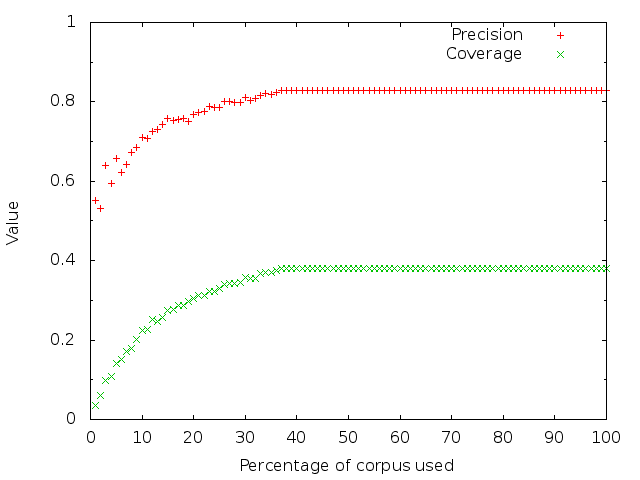
\includegraphics[width=0.45\textwidth]{fig/slot-predicate-percents.png}
    \caption{\label{fig:fonction_predicate}Performance du modèle fonction-prédicat en entraînant le modèle sur une sous-partie du corpus : de 0 à 100~\%.}
\end{figure}

La figure~\ref{fig:fonction_predicate} montre que ce niveau de performance ne
demande pas un gros corpus. C'est un enseignement intéressant pour deux
raisons~:

\begin{itemize}

    \item Un corpus de petite taille suffit pour obtenir cette performance, ce
    qui est adapté à des domaines où les corpus même non annotés peuvent être
    petits.

    \item L'algorithme ne fait pas de sur-apprentissage en ayant un biais fort
    et une variance faible, ce qui est souhaitable ici.

\end{itemize}

\subsection{Comparaison avec SEMAFOR}

% TODO scores sont en XX
SEMAFOR \citep{das2014frame} est la référence actuelle en annotation en rôle
sémantiques supervisée : c'est le système qui obtient les meilleurs résultats
sur le corpus full-text de FrameNet 1.5. Toutes les parties du discours sont
annotées alors que nous ne nous concentrons que sur les verbes. Sur la tâche
complète, SEMAFOR obtient un score F1 de XX~\%, score à comparer avec les XX\~
de notre système. Le système de SEMAFOR découpe la tâche en trois parties :

\begin{itemize}
    \item identification des prédicats déclencheurs
    \item identification des frames FrameNet
    \item identification des arguments et annotation en rôles sémantiques 
\end{itemize}

Une comparaison directe n'est pas possible étant donné que les tâches sont
découpées différemment dans notre système. Cependant, il est intéressant de
noter l'importance des données d'entraînement : pour l'identification des
frames FrameNet avec des prédicats de la vérité-terrain\footnote{les résultats
pour des déclencheurs identifiés manuellement n'ont été donnés que pour le
corpus SemEval, un sous-ensemble du corpus FrameNet 1.5 complet}, les mêmes
modèles grimpent de 74.21~\% à 90.51~\% quand la taille du corpus augmente en
passant du corpus SemEval (XXX phrases) au corpus FrameNet 1.5 (XXX phrases).
De la même manière pour l'identification des arguments avec des frames FrameNet
de la vérité-terrain, les résultats augmentent de 48.09~\% 68.83~\%. C'est très
encourageant pour les domaines disposant de très gros corpus, mais suggère que
d'autres solutions sont à identifier pour les domaines où de tels corpus ne
sont pas disponibles.

\section{Travaux futurs}

Nous avons appliqué ce travail à des domaines spécifiques et variés : football,
réchauffement climatique et informatique (Chapitre~\ref{ch:domainsrl}).

Nous pensons aussi prendre en compte la similarité entre les remplisseurs déjà
identifiés et les remplisseurs pour lesquels un rôle reste encore à identifier
afin d'améliorer nos modèles de probabilité. En effet, l'information des cadres
de sous-catégorisation est cruciale pour identifier les arguments, mais
l'information sémantique concernant le contenu des remplisseurs est aussi utile
pour déterminer le rôle correct.
% TODO ref vers chapitre similarité ASFALDA

Enfin, de la même manière que la prise en compte de la voix passive a amélioré
les résultats, d'autres phénomènes de syntaxe profonde doivent être pris en
compte. La coordination est une autre source commune d'erreur. En effet, quand
deux verbes partagent le même sujet, une analyse syntaxique profonde indique à
chaque fois quel est le sujet profond. Voici deux exemples tirés du corpus
FrameNet :

\begin{itemize}
    \item You are not fair when you belittle Sheik Bin Baz 's blunder and
          exaggerate the one by Sheik Maqdasi ...
    \item Hostile and even friendly nations routinely steal information from
          U.S. companies and share it with their own companies
\end{itemize}

L'objectif est de traiter ces phénomènes de manière plus générale en intégrant
le système de \cite{ribeyre2013systeme} qui permet de prendre en compte de
nouveaux phénomènes en ajoutant de nouvelles règles au système. Ainsi, les
différents phénomènes seront prise en compte de manière cohérente.

\section{Conclusion}

Nous avons implémenté un système d'annotation en rôles sémantiques basé sur la
connaissance. Nous avons utilisé des outils et des corpus disponibles
publiquement qui rendent notre travail facilement reproductible et facilitent
le travail de comparaison, maintenant et dans le futur. Nous avons commencé à
améliorer le système initial, montrant son potentiel. L'indépendance de
l'approche par rapport au corpus considéré la rend attractive pour annoter des
domaines ne disposant que de peu ou pas de corpus annotés en rôles sémantiques.
